\section{Discrepancies and Ambiguities}
\label{discrep}

% Moved earlier to display nicely in paper
% \discrepsTable{}

After gathering all this data\footnote{Available in \texttt{ApproachGlossary.csv}
    and \texttt{QualityGlossary.csv} at \ifblind{[Repository link suppressed]}
    {\url{https://github.com/samm82/TestGen-Thesis}}.}, we found many discrepancies
and ambiguities. A summary of these is shown in
\refDiscrepsTable{}, where a given row corresponds to the number of
discrepancies either within that category and/or with a ``more trusted''
\hyperref[sources]{source category} (i.e., a previous row in the table). Issues
with \nameref{syns}, \nameref{par-rels}, and \nameref{categories-discrep} are
(Exp)licit or (Imp)licit. Issues with \nameref{func-test-discrep},
\ifnotpaper\nameref{oat-discrep}\else\acf{operat}\footnote{Section omitted for
        brevity.}\fi, \nameref{recov-discrep}, and \nameref{scal-discrep} are
also given, although not listed separately in \refDiscrepsTable{}; these
are counted alongside \nameref{other-discrep}, all grouped into
degrees of severity as follows\ifnotpaper:\else.
(Note that only select discrepancies are listed for brevity.) \fi

\begin{itemize}
    \item High: Semantic differences between test approaches
    \item (Med)ium: Differences in supporting information about test approaches
    \item Low: Typos, redundancy, or issues with referencing
\end{itemize}

\ifnotpaper \begin{figure*}
\centering
\begin{subfigure}[t]{0.475\textwidth}
\begin{tikzpicture}[thick, scale=0.7, every label/.style={align=left, scale=0.7}]
   \pie[text=legend, sum=auto, hide number, color={blue!60, cyan!60, yellow!60}]{
      25/48.1\%,
      22/42.3\%,
      5/9.6\%
}
\end{tikzpicture}
\caption{Discrepancies found in \stds{}.}
\label{fig:stdDiscrepSources}
\end{subfigure}
\hfill
\begin{subfigure}[t]{0.475\textwidth}
\begin{tikzpicture}[thick, scale=0.7, every label/.style={align=left, scale=0.7}]
   \pie[text=legend, sum=auto, hide number, color={blue!60, yellow!60, orange!60}]{
      24/38.1\%,
      29/46\%,
      10/15.9\%
}
\end{tikzpicture}
\caption{Discrepancies found in \metas{}.}
\label{fig:metaDiscrepSources}
\end{subfigure}
\vskip\baselineskip
\begin{subfigure}[t]{0.475\textwidth}
\begin{tikzpicture}[thick, scale=0.7, every label/.style={align=left, scale=0.7}]
   \pie[text=legend, sum=auto, hide number, color={blue!60, yellow!60, orange!60, red!60}]{
      7/21.9\%,
      13/40.6\%,
      7/21.9\%,
      5/15.6\%
}
\end{tikzpicture}
\caption{Discrepancies found in \texts{}.}
\label{fig:textDiscrepSources}
\end{subfigure}
\hfill
\begin{subfigure}[t]{0.475\textwidth}
\begin{tikzpicture}[thick, scale=0.7, every label/.style={align=left, scale=0.7}]
   \pie[text=legend, sum=auto, hide number, color={blue!60, yellow!60, orange!60, red!60, blue!60!cyan!60}]{
      14/26.9\%,
      17/32.7\%,
      14/26.9\%,
      3/5.8\%,
      4/7.7\%
}
\end{tikzpicture}
\caption{Discrepancies found in \papers{}.}
\label{fig:paperDiscrepSources}
\end{subfigure}
\vskip\baselineskip
\begin{center}
\begin{subfigure}[t]{\linewidth}
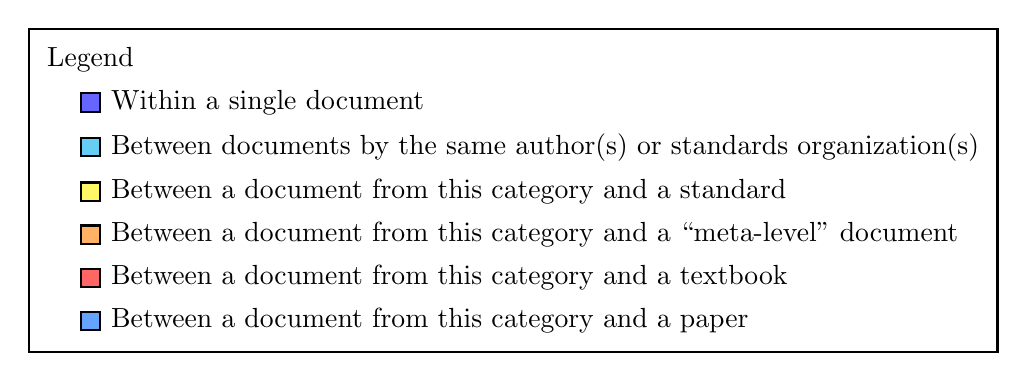
\begin{tikzpicture}
\matrix [thick, draw=black] {
\node[label=center:Legend] {{}}; \\
\node[thick, shape=rectangle, draw=black, fill=blue!60, label=right:{Within a single document}](0) {}; \\
\node[thick, shape=rectangle, draw=black, fill=cyan!60, label=right:{Between documents by the same author(s) or standards organization(s)}](1) {}; \\
\node[thick, shape=rectangle, draw=black, fill=yellow!60, label=right:{Between a document from this category and a standard}](2) {}; \\
\node[thick, shape=rectangle, draw=black, fill=orange!60, label=right:{Between a document from this category and a ``meta-level'' document}](3) {}; \\
\node[thick, shape=rectangle, draw=black, fill=red!60, label=right:{Between a document from this category and a textbook}](4) {}; \\
\node[thick, shape=rectangle, draw=black, fill=blue!60!cyan!60, label=right:{Between a document from this category and a paper}](5) {}; \\
};
\end{tikzpicture}
\end{subfigure}
\end{center}
\hfill
\caption{Sources of discrepancies based on \hyperref[sources]{source category}.}
\label{fig:discrepSources}
\end{figure*}
 \fi

\subsection{Synonyms}
\label{syns}
The same approach often has many names. For example,
\emph{specification-based testing} is also called\todo{more in Umar2000}:
\begin{enumerate}
    \item Black-Box Testing
          \ifnotpaper
              (\citealp[p.~9]{IEEE2022}; \citeyear[p.~8]{IEEE2021};
              \citeyear[p.~431]{IEEE2017}; \citealp[p.~5-10]{SWEBOK2024};
              \citealpISTQB{}; \citealp[p.~46]{Firesmith2015} (without hyphen);
              \citealp[p.~344]{SakamotoEtAl2013}; \citealp[p.~399]{vanVliet2000})
          \else
              \cite[p.~431]{IEEE2017}, \cite{ISTQB}, \cite[p.~5-10]{SWEBOK2024},
              \cite[p.~9]{IEEE2022}, \cite[p.~399]{vanVliet2000},
              \cite[p.~8]{IEEE2021},
              % \cite[p.~46]{Firesmith2015} (without hyphen),
              \cite[p.~344]{SakamotoEtAl2013}
          \fi
    \item Closed-Box Testing
          \ifnotpaper
              (\citealp[p.~9]{IEEE2022}; \citeyear[p.~431]{IEEE2017})
          \else
              \cite[p.~431]{IEEE2017}, \cite[p.~9]{IEEE2022}
          \fi
    \item Functional Testing\footnote{This may be an outlier; see
              \Cref{spec-func-test}.}
          \ifnotpaper
              (\citeyear[p.~196]{IEEE2017}; \citealp[p.~44]{Kam2008};
              \citealp[p.~399]{vanVliet2000}; implied by \citeyear[p.~129]{IEEE2021};
              \citeyear[p.~431]{IEEE2017})
          \else
              \cite[p.~196]{IEEE2017}, \cite[p.~399]{vanVliet2000},
              \cite[p.~44]{Kam2008}
          \fi
    \item Domain Testing \citep[p.~5-10]{SWEBOK2024}
          \ifnotpaper
    \item Input Domain-Based Testing (implied by \citep[p.~4-8]{SWEBOK2014})
          \fi
\end{enumerate}

While some of these synonyms may express mild variations, their core meaning
is nevertheless the same. Here we use the terms ``specification-based'' and
``structure-based testing'' as they articulate the source of the information
for designing test cases, but a team or project also using gray-box testing may
prefer the terms ``black-box'' and ``white-box testing'' for consistency.
Thus, synonyms do not inherently signify a discrepancy. Unfortunately, there
are many instances of incorrect or ambiguous synonyms, such as the following:

\begin{enumerate}
    \item \ifnotpaper\citeauthor{SneedAndGöschl2000} give \else Reference
              \cite{SneedAndGöschl2000} gives \fi ``white-'', ``grey-'', and
          ``black-box testing'' as synonyms for ``module'', ``integration'',
          and ``system testing'', respectively%
          \ifnotpaper\ \citeyearpar[p.~18]{SneedAndGöschl2000}\todo{OG Hetzel88}\fi, but
          this mapping is incorrect; black-box testing can be performed on a
          module, for example\todo{find source}. This makes the claim that
          ``red-box testing'' is a synonym for ``acceptance testing''
          \citetext{p.~18} lose credibility.
    \item ``Program testing'' is given as a synonym of ``component testing''
          \citep[p.~46]{Kam2008}, although it probably should be a synonym of
          ``system testing'' instead.
    \item \ifnotpaper\citeauthor{Kam2008} \else Reference \cite{Kam2008} \fi
          seems to imply that ``mutation testing'' is a
          synonym of ``back-to-back testing''%
          \ifnotpaper\ \citeyearpar[p.~46]{Kam2008}\fi,
          but these are two quite distinct techniques.
    \item ``Conformance testing'' is implied to be a synonym of ``compliance
          testing'' by \ifnotpaper\citeauthor{Kam2008}\else\cite{Kam2008}\fi,
          which only makes sense because
          of the vague definition of ``compliance testing'': ``testing to
          determine the compliance of the component or system''
          \ifnotpaper\citeyearpar[p.~43]{Kam2008}\else\citetext{p.~43}\fi.
\end{enumerate}

\phantomsection{}
\label{multiSyns}
There are also cases in which a term is given a synonym to two (or more)
disjoint, unrelated terms, which would be a source of ambiguity to teams using
these terms. Ten of these cases were identified through automatic analysis of
the generated graphs\ifnotpaper, listed below\else. The following four are the
most prominent examples\fi:

% Moved here to display nicely in paper
\ifnotpaper\else\def\specfn{\footnote{See \Cref{spec-func-test}.}}

\begin{paperTable}
    \centering
    \caption{Pairs of test approaches with both parent-child and synonym relations.}
    \label{tab:parSyns}
    \begin{minipage}{\linewidth}
        \centering
        \begin{tabular}{|rcl|l|l|}
            \hline
            \thead{``Child''}        & \thead{$\to$} & \thead{``Parent''}                       & \thead{Parent-Child Source(s)}                                        & \thead{Synonym Source(s)}                                                   \\
            \hline
            All Transitions Testing  & $\to$         & State Transition Testing                 & \citep[p.~19]{IEEE2021}                                               & \citep[p.~15]{Kam2008}                                                      \\
            Co-existence Testing     & $\to$         & Compatibility Testing                    & \cite[p.~3]{IEEE2022}, \cite{ISO_IEC2023a}, \cite[Tab.~A.1]{IEEE2021} & \citep[p.~37]{IEEE2021}                                                     \\
            Fault Tolerance Testing  & $\to$         & Robustness Testing\footnote{\ftrnote{F}} & \citep[p.~56]{Firesmith2015}                                          & \citepISTQB{}                                                               \\
            Functional Testing       & $\to$         & Specification-based Testing\specfn       & \citep[p.~38]{IEEE2021}                                               & \cite[p.~196]{IEEE2017}, \cite[p.~399]{vanVliet2000}, \cite[p.~44]{Kam2008} \\
            Orthogonal Array Testing & $\to$         & Pairwise Testing                         & \citep[p.~1055]{Mandl1985}                                            & \cite[p.~5-11]{SWEBOK2024}, \cite[p.~473]{Valcheva2013}                     \\
            Performance Testing      & $\to$         & Performance-related Testing              & \cite[p.~22]{IEEE2022}, \cite[p.~38]{IEEE2021}                        & \citep[p.~1187]{Moghadam2019}                                               \\
            Use Case Testing         & $\to$         & Scenario Testing                         & \cite[p.~20]{IEEE2021}\todo{OG Hass, 2008}                            & \cite{ISTQB}, \cite[pp.~47-49]{Kam2008}                                     \\
            \hline
        \end{tabular}
    \end{minipage}
\end{paperTable}
\fi

\begin{enumerate}
    \ifnotpaper \item \textbf{Invalid Testing:}
\begin{itemize}
    \item Error Tolerance Testing \citep[p.~45]{Kam2008}
    \item Negative Testing \ifnotpaper
              (\citealpISTQB{}; implied by \citealp[p.~10]{IEEE2021}) \else
              \citep{ISTQB} (implied by \citep[p.~10]{IEEE2021}) \fi
\end{itemize}
\item \textbf{Soak Testing:}
\begin{itemize}
    \item Endurance Testing \citep[p.~39]{IEEE2021}
    \item Reliability Testing\ifnotpaper\
              (\citealp[Tab.~2]{Gerrard2000a}; \citeyear[Tab.~1,~p.~26]{Gerrard2000b})
          \else\footnote{Endurance testing is given as a kind of reliability
                  testing by \citet[p.~55]{Firesmith2015}, although the terms
                  are not synonyms.} \citep[Tab.~1,~p.~26]{Gerrard2000b},
              \citep[Tab.~2]{Gerrard2000a}\fi
\end{itemize}
\item \textbf{User Scenario Testing:}
\begin{itemize}
    \item Scenario Testing \citepISTQB{}
    \item Use Case Testing\ifnotpaper\ \else\footnote{``Scenario testing'' and
                  ``use case testing'' are given as synonyms by \citepISTQB{}
                  and \citep[pp.~47-49]{Kam2008}
                  but listed separately by \citep[p.~22]{IEEE2022}, \ifnotpaper who
                      also give \else which also gives \fi ``use case testing'' as a
                  ``common form of scenario testing'' \citep[p.~20]{IEEE2021}.
                  This implies that ``use case testing'' may instead be a child of
                  ``user scenario testing'' (see \Cref{tab:parSyns}).}\fi
          \citep[p.~48]{Kam2008} (although ``an actor can be a user or another
          system'' \citep[p.~20]{IEEE2021})
\end{itemize}
\item \textbf{Link Testing:}
\begin{itemize}
    \item Branch Testing (implied by \citealp[p.~24]{IEEE2021})
    \item Component Integration Testing \citep[p.~45]{Kam2008}
    \item Integration Testing (implied by \citealp[p.~13]{Gerrard2000a})
\end{itemize} \else \item \textbf{Invalid Testing:}
\begin{itemize}
    \item Error Tolerance Testing \citep[p.~45]{Kam2008}
    \item Negative Testing \ifnotpaper
              (\citealpISTQB{}; implied by \citealp[p.~10]{IEEE2021}) \else
              \citep{ISTQB} (implied by \citep[p.~10]{IEEE2021}) \fi
\end{itemize}
\item \textbf{Soak Testing:}
\begin{itemize}
    \item Endurance Testing \citep[p.~39]{IEEE2021}
    \item Reliability Testing\ifnotpaper\
              (\citealp[Tab.~2]{Gerrard2000a}; \citeyear[Tab.~1,~p.~26]{Gerrard2000b})
          \else\footnote{Endurance testing is given as a kind of reliability
                  testing by \citet[p.~55]{Firesmith2015}, although the terms
                  are not synonyms.} \citep[Tab.~1,~p.~26]{Gerrard2000b},
              \citep[Tab.~2]{Gerrard2000a}\fi
\end{itemize}
\item \textbf{User Scenario Testing:}
\begin{itemize}
    \item Scenario Testing \citepISTQB{}
    \item Use Case Testing\ifnotpaper\ \else\footnote{``Scenario testing'' and
                  ``use case testing'' are given as synonyms by \citepISTQB{}
                  and \citep[pp.~47-49]{Kam2008}
                  but listed separately by \citep[p.~22]{IEEE2022}, \ifnotpaper who
                      also give \else which also gives \fi ``use case testing'' as a
                  ``common form of scenario testing'' \citep[p.~20]{IEEE2021}.
                  This implies that ``use case testing'' may instead be a child of
                  ``user scenario testing'' (see \Cref{tab:parSyns}).}\fi
          \citep[p.~48]{Kam2008} (although ``an actor can be a user or another
          system'' \citep[p.~20]{IEEE2021})
\end{itemize}
\item \textbf{Link Testing:}
\begin{itemize}
    \item Branch Testing (implied by \citealp[p.~24]{IEEE2021})
    \item Component Integration Testing \citep[p.~45]{Kam2008}
    \item Integration Testing (implied by \citealp[p.~13]{Gerrard2000a})
\end{itemize} \fi
\end{enumerate}

\subsection{Parent Relations}
\label{par-rels}

Parent relations are not immune to difficulties, including self-referential
definitions\footnote{Since these are by nature self-contained within a given
    source, these are counted \emph{once} as explicit discrepancies within
    their sources in \Cref{tab:discreps}.}, which were identified
through automatic analysis of the generated graphs.
\ifnotpaper \input{build/selfCycles} Performance
\else Performance and usability testing are both given as sub-approaches of
    themselves \cite[Tab.~1]{Gerrard2000b}, \cite[Tab.~2]{Gerrard2000a},
    while performance \fi
testing is \emph{not} described as a sub-approach of usability testing%
\ifnotpaper\ by \citep{Gerrard2000a, Gerrard2000b}, which \else. This
\fi would have been more meaningful information to capture.

There are also pairs of synonyms where one is described as a
sub-approach of the other, abusing the meaning of ``synonym'' and
causing confusion. We identified \parSynCount{} of these pairs through automatic
analysis of the generated graphs, which are given in \Cref{tab:parSyns}.
\ifnotpaper Finally, it is worth pointing out that \ftrnote{f}

    \begin{landscape}
        \discrepsTable{}
        \def\specfn{\footnote{See \Cref{spec-func-test}.}}

\begin{paperTable}
    \centering
    \caption{Pairs of test approaches with both parent-child and synonym relations.}
    \label{tab:parSyns}
    \begin{minipage}{\linewidth}
        \centering
        \begin{tabular}{|rcl|l|l|}
            \hline
            \thead{``Child''}        & \thead{$\to$} & \thead{``Parent''}                       & \thead{Parent-Child Source(s)}                                        & \thead{Synonym Source(s)}                                                   \\
            \hline
            All Transitions Testing  & $\to$         & State Transition Testing                 & \citep[p.~19]{IEEE2021}                                               & \citep[p.~15]{Kam2008}                                                      \\
            Co-existence Testing     & $\to$         & Compatibility Testing                    & \cite[p.~3]{IEEE2022}, \cite{ISO_IEC2023a}, \cite[Tab.~A.1]{IEEE2021} & \citep[p.~37]{IEEE2021}                                                     \\
            Fault Tolerance Testing  & $\to$         & Robustness Testing\footnote{\ftrnote{F}} & \citep[p.~56]{Firesmith2015}                                          & \citepISTQB{}                                                               \\
            Functional Testing       & $\to$         & Specification-based Testing\specfn       & \citep[p.~38]{IEEE2021}                                               & \cite[p.~196]{IEEE2017}, \cite[p.~399]{vanVliet2000}, \cite[p.~44]{Kam2008} \\
            Orthogonal Array Testing & $\to$         & Pairwise Testing                         & \citep[p.~1055]{Mandl1985}                                            & \cite[p.~5-11]{SWEBOK2024}, \cite[p.~473]{Valcheva2013}                     \\
            Performance Testing      & $\to$         & Performance-related Testing              & \cite[p.~22]{IEEE2022}, \cite[p.~38]{IEEE2021}                        & \citep[p.~1187]{Moghadam2019}                                               \\
            Use Case Testing         & $\to$         & Scenario Testing                         & \cite[p.~20]{IEEE2021}\todo{OG Hass, 2008}                            & \cite{ISTQB}, \cite[pp.~47-49]{Kam2008}                                     \\
            \hline
        \end{tabular}
    \end{minipage}
\end{paperTable}

    \end{landscape}
\else % Moved earlier to display nicely in paper
\fi

\subsection{Categories of Testing Approaches}
\label{categories-discrep}
While the IEEE categorization of testing approaches is useful, it
is not without its faults. The boundaries between items within a category may
be unclear: ``although each technique is defined independently of all others,
in practice [sic] some can be used in combination with other techniques''
\citep[p.~8]{IEEE2021}. For example, ``the test coverage items derived by
applying equivalence partitioning can be used to identify the input parameters
of test cases derived for scenario testing'' \citetext{p.~8}. Even the categories
themselves are not consistently defined, and some approaches are categorized
differently by different sources:

% ; these differences are tracked so
% they can be analyzed more systematically\seeThesisIssuePar{21}.

\begin{enumerate}
    \item % Discrep count: {IEEE2022}
          \ifnotpaper \citeauthor{IEEE2022} \else ISO/IEC and IEEE \fi
          categorize experience-based testing as both a test design
          technique and a test practice on the same page---twice
          \ifnotpaper \citeyearpar[Fig.~2,~p.~34]{IEEE2022}\else
              \cite[Fig.~2,~p.~34]{IEEE2022}\fi!
          \ifnotpaper
              \begin{itemize}
                  \item % Discrep count: {IEEE2021} | {IEEE2022} {IEEE2021} {SWEBOK2024} ISTQB
                        These authors previously say ``experience-based testing
                        practices like exploratory testing \dots\ are not
                        \dots\ techniques for designing test cases'', although
                        they ``can use \dots\ test techniques''
                        \citeyearpar[p.~viii]{IEEE2021}. This implies that
                        ``experience-based test design techniques'' are
                        techniques used by the \emph{practice} of experience-based
                        testing, not that experience-based testing is
                        \emph{itself} a test technique. If this is the case, it
                        is not always clearly articulated
                        \ifnotpaper
                            (\citealp[pp.~4,~22]{IEEE2022}; \citeyear[p.~4]{IEEE2021};
                            \citealp[p.~5-13]{SWEBOK2024}; \citealpISTQB{})
                        \else
                            \cite[pp.~4,~22]{IEEE2022}, \cite[p.~4]{IEEE2021},
                            \cite[p.~5-13]{SWEBOK2024}, \cite{ISTQB}
                        \fi
                        and is
                        sometimes contradicted \citep[p.~46]{Firesmith2015}.
                        However, this conflates the distinction between
                        ``practice'' and ``technique'', making these terms less
                        useful, so this may just be a mistake\seeThesisIssuePar{64}.

                        % Furthermore, if a ``class of \dots\ techniques''
                        % is a practice, then other ``techniques'', such as combinatorial testing
                        % (\citealp[pp.~3,~22]{IEEE2022}; \citeyear[p.~2]{IEEE2021};
                        % \citealp[p.~5-11]{SWEBOK2024}; \citealpISTQB{}), data flow testing
                        % (\citealp[p.~22]{IEEE2022}; \citeyear[p.~3]{IEEE2021};
                        % \citealp[p.~5-13]{SWEBOK2024}; \citealp[p.~43]{Kam2008}), performance(-related)
                        % testing (\citealp[p.~38]{IEEE2021}; \citealp[p.~1187]{Moghadam2019}), and
                        % security testing \citep[p.~40]{IEEE2021} may \emph{also}
                        % actually be practices, since they are also described as classes or families of
                        % techniques. The same could be said of the more
                        % general specification- and structure-based testing, especially since these,
                        % plus experience-based testing, are described as ``complementary'' \citetext{p.~8,~Fig.~2}.
                        % % \citeyearpar[p.~8, Fig.~2]{IEEE2021}

                  \item % Discrep count: {IEEE2022}
                        % Discrep count: {IEEE2022} {IEEE2021} | {SWEBOK2024}
                        This also causes confusion about its children, such as
                        error guessing and exploratory testing; again, on the
                        same page,
                        \ifnotpaper
                            \citeauthor{IEEE2022} say
                        \else
                            \cite[p.~34]{IEEE2022} says
                        \fi error guessing is
                        an ``experience-based test design technique'' and
                        ``experience-based test practices include \dots\
                        exploratory testing, tours, attacks, and
                        checklist-based testing''%
                        \ifnotpaper{ \citeyearpar[p.~34]{IEEE2022}.}
                        \else{.}
                        \fi
                        Other sources also do not agree whether error guessing
                        is a technique
                        \ifnotpaper
                            (pp.~20,~22; \citeyear[p.~viii]{IEEE2021})
                        \else
                            \cite[pp.~20,~22]{IEEE2022}, \cite[p.~viii]{IEEE2021}
                        \fi
                        or a practice \citep[p.~5-14]{SWEBOK2024}.
              \end{itemize}
          \fi
    \item The following test approaches are categorized as test
          techniques by \citep[p.~38]{IEEE2021} and as test types by the
          sources provided:
          \begin{enumerate}
              \item % Discrep count: {IEEE2021} | {IEEE2022} {IEEE2013} implied by {ISO_IEC2023a} {IEEE2021} {Firesmith2015}
                    Capacity testing
                    \ifnotpaper
                        (\citealp[p.~22]{IEEE2022};
                        \citeyear[p.~2]{IEEE2013}; implied by its quality
                        (\citealp{ISO_IEC2023a}; \citealp[Tab.~A.1]{IEEE2021})
                        and by \citep[p.~53]{Firesmith2015})%
                    \else
                        \cite[p.~22]{IEEE2022}, \cite[p.~2]{IEEE2013}%
                    \fi,
              \item % Discrep count: {IEEE2021} | {IEEE2013} implied by {Firesmith2015}
                    Endurance testing
                    \ifnotpaper
                        (\citealp[p.~2]{IEEE2013};
                        implied by \citep[p.~55]{Firesmith2015})%
                    \else
                        \cite[p.~2]{IEEE2013}%
                    \fi,
              \item % Discrep count: {IEEE2021} | {IEEE2022} {IEEE2017} {IEEE2013} ISTQB implied by {Firesmith2015}
                    Load testing
                    \ifnotpaper
                        (\citealp[pp.~5,~20,~22]{IEEE2022};
                        \citeyear[p.~253]{IEEE2017}\todo{OG IEEE 2013};
                        \citealpISTQB{}; implied by \citep[p.~54]{Firesmith2015})%
                    \else
                        \cite[p.~253]{IEEE2017}\todo{OG IEEE 2013},
                        \cite{ISTQB}, \cite[pp.~5,~20,~22]{IEEE2022}%
                    \fi,
              \item % Discrep count: {IEEE2021} | {IEEE2022} {IEEE2021} implied by {Firesmith2015}
                    Performance testing
                    \ifnotpaper
                        (\citealp[pp.~7,~22,~26-27]{IEEE2022};
                        \citeyear[p.~7]{IEEE2021}; implied by
                        \citep[p.~53]{Firesmith2015})%
                    \else
                        \cite[pp.~7,~22,~26-27]{IEEE2022}, \cite[p.~7]{IEEE2021}%
                    \fi, and
              \item % Discrep count: {IEEE2021} | {IEEE2022} {IEEE2017} implied by {Firesmith2015}
                    Stress testing
                    \ifnotpaper
                        (\citealp[pp.~9,~22]{IEEE2022};
                        \citeyear[p.~442]{IEEE2017}; implied by
                        \citep[p.~54]{Firesmith2015})%
                    \else
                        \cite[p.~442]{IEEE2017}, \cite[pp.~9,~22]{IEEE2022}%
                    \fi.
          \end{enumerate}
    \item % Discrep count: {IEEE2022} {IEEE2021} | {PetersAndPedrycz2000}
          ``Installability testing'' is given as a test type
          \ifnotpaper
              (\citealp[p.~22]{IEEE2022}; \citeyear[p.~38]{IEEE2021})
          \else
              \cite[p.~22]{IEEE2022}, \cite[p.~38]{IEEE2021}
          \fi but is sometimes called a test level as
          ``installation testing'' \citep[p.~445]{PetersAndPedrycz2000}.
    \item % Discrep count: {IEEE2022} {IEEE2021} | {Kam2008} implied by {IEEE2021} {IEEE2017}
          Model-based testing is categorized as both a test practice
          \ifnotpaper
              (\citealp[p.~22]{IEEE2022}; \citeyear[p.~viii]{IEEE2021})
          \else
              \cite[p.~22]{IEEE2022}, \cite[p.~viii]{IEEE2021}
          \fi and a test technique
          \ifnotpaper
              (\citealp[p.~4]{Kam2008}; implied by
              \citealp[p.~7]{IEEE2021}; \citeyear[p.~469]{IEEE2017})%
          \else
              \cite[p.~4]{Kam2008}%
          \fi.
    \item % Discrep count: {IEEE2022} | {Kam2008}
          Data-driven testing is categorized as both a test practice
          \citep[p.~22]{IEEE2022} and a test technique
          \citep[p.~43]{Kam2008}\todo{OG Fewster and Graham}.
    \item % Discrep count: {SWEBOK2024} | {Kam2008}
          Although ad hoc testing is sometimes classified as a ``technique''
          \citep[p.~5-14]{SWEBOK2024}, it is one in which ``no recognized test
          design technique is used'' \citep[p.~42]{Kam2008}.
\end{enumerate}

There are also instances of inconsistencies between parent and child
test approach categorizations. This may indicate they aren't necessarily the
same, or that more thought must be given to this method of classification.

\subsection{Functional Testing}
\label{func-test-discrep}

``Functional testing'' is described alongside many other, likely related,
terms. This leads to confusion about what distinguishes these terms, as shown
by the following five:

\subsubsection{Specification-based Testing}
\label{spec-func-test}
This is defined as ``testing in which the principal test basis is the external
inputs and outputs of the test item'' \citep[p.~9]{IEEE2022}. This agrees
with a definition of ``functional testing'': ``testing that
\dots\ focuses solely on the outputs generated in response to
selected inputs and execution conditions'' \citep[p.~196]{IEEE2017}.
\todo{\citet[p.~399]{vanVliet2000} may list these as synonyms; investigate}
Notably, \citet{IEEE2017} lists both as synonyms of
``black-box testing'' \citetext{pp. 431, 196, respectively}, despite them
sometimes being defined separately. For example, the \acf{istqb} defines
``specification-based testing'' as ``testing based on an analysis of the
specification of the component or system'' \ifnotpaper (and gives ``black-box
    testing'' as a synonym) \fi and ``functional testing'' as ``testing
performed to evaluate if a component or system satisfies functional
requirements'' \ifnotpaper (specifying no synonyms) \citepISTQB{};
    % Discrep count (SYNS): {IEEE2022} {IEEE2017} | ISTQB
    the latter references \citet[p.~196]{IEEE2017}
    (``testing conducted to evaluate the compliance of a system or
    component with specified functional requirements'') which
    \emph{has} ``black-box testing'' as a synonym, and mirrors
    \citet[p.~21]{IEEE2022} (testing ``used to check the implementation
    of functional requirements'')\else \cite{ISTQB}\fi. Overall,
specification-based testing \citep[pp.~2-4,~6-9,~22]{IEEE2022} \ifnotpaper and
    black-box testing (\citealp[p.~5-10]{SWEBOK2024};
    \citealp[p.~3]{SouzaEtAl2017})
    % \else \cite[p.~3]{SouzaEtAl2017}, \cite[p.~5-10]{SWEBOK2024}
    are test design techniques \else is a test design technique \fi used to
``derive corresponding test cases'' \citep[p.~11]{IEEE2022} from
``selected inputs and execution conditions'' \citep[p.~196]{IEEE2017}.

\subsubsection{Correctness Testing}
\ifnotpaper \citeauthor{SWEBOK2024} \else The \acs{swebok} V4 \fi says
``test cases can be designed to check that the functional
specifications are correctly implemented, which is variously
referred to in the literature as conformance testing, correctness
testing or functional testing'' \ifnotpaper \citeyearpar[p.~5-7]{SWEBOK2024}%
\else \cite[p.~5-7]{SWEBOK2024}\fi; this mirrors previous definitions
of ``functional testing'' \ifnotpaper (\citealp[p.~21]{IEEE2022};
    \citeyear[p.~196]{IEEE2017}) \else \cite[p.~196]{IEEE2017},
    \cite[p.~21]{IEEE2022} \fi but groups it with ``correctness
testing''. Since ``correctness'' is a software quality \ifnotpaper
    (\citealp[p.~104]{IEEE2017}; \citealp[p.~3-13]{SWEBOK2024}) \else
    \cite[p.~104]{IEEE2017}, \cite[p.~3-13]{SWEBOK2024} \fi which is
what defines a ``test type'' \citep[p.~15]{IEEE2022}\seeParAlways{qual-test},
it seems consistent to label ``functional testing'' as a ``test type''
\citep[pp.~15,~20,~22]{IEEE2022}; this conflicts with its categorization
as a ``technique'' if considered a synonym of \nameref{spec-func-test}.
% Discrep count (CATS): implied by {IEEE2017} {SWEBOK2024} {IEEE2022} | {IEEE2022} {SWEBOK2024} {SouzaEtAl2017} {IEEE2017}
``Correctness testing'' is listed separately from ``functionality testing'' by
\citet[p.~53]{Firesmith2015}.
% Discrep count (SYNS): {SWEBOK2024} | {Firesmith2015}

\subsubsection{Conformance Testing}
Testing that ensures ``that the functional specifications are correctly
implemented'', and can be called ``conformance testing'' or ``functional
testing'' \citep[p.~5-7]{SWEBOK2024}.
``Conformance testing'' is later defined as testing used ``to
verify that the \acs{sut} conforms to standards, rules,
specifications, requirements, design, processes, or practices''
\citep[p.~5-7]{SWEBOK2024}. This definition seems to be a superset
of testing methods mentioned earlier as the latter includes ``standards,
rules, requirements, design, processes, \dots\ [and]'' practices in
\emph{addition} to specifications!
% Discrep count (SYNS): {SWEBOK2024} | implied by {SWEBOK2024}

A complicating factor is that ``compliance testing'' is also
(plausibly) given as a synonym of ``conformance testing''
\citep[p.~43]{Kam2008}. However, ``conformance
testing'' can also be defined as testing that evaluates the degree
to which ``results \dots\ fall within the limits that define
acceptable variation for a quality requirement''
\citep[p.~93]{IEEE2017}\todo{OG PMBOK 5th ed.}, which seems to
describe something different.
% Discrep count (SYNS): {Kam2008} | implied by {IEEE2017}

% TODO: pull out into Recommendations
% Perhaps this second definition of
% ``conformance testing'' should be used, and the previous definition
% of ``compliance testing'' should be used for describing compliance with
% external standards, rules, etc.~to keep them distinct.

\subsubsection{Functional Suitability Testing}
Procedure testing is
called a ``type of functional suitability testing''
\citep[p.~7]{IEEE2022}, but no definition of that term is given.
``Functional suitability'' is the
``capability of a product to provide functions that meet stated and
implied needs of intended users when it is used under specified
conditions'', including meeting ``the functional specification''
\citep{ISO_IEC2023a}. This seems to align with the definition of
``functional testing'' as related to ``black-box/%
specification-based testing''.
\ifnotpaper
    ``Functional suitability'' has
    three child terms: ``functional completeness'' (the ``capability of
    a product to provide a set of functions that covers all the
    specified tasks and intended users' objectives''), ``functional
    correctness'' (the ``capability of a product to provide accurate
    results when used by intended users''), and ``functional
    appropriateness'' (the ``capability of a product to provide
    functions that facilitate the accomplishment of specified tasks and
    objectives'') \citep{ISO_IEC2023a}. Notably, ``functional
    correctness'', which includes precision and accuracy
    (\citealp{ISO_IEC2023a}; \citealpISTQB{}), \else ``Functional
    correctness'', a child of ``functional suitability'', is the ``capability
    of a product to provide accurate results when used by intended users''
    \cite{ISO_IEC2023a} and \fi seems to align with
the quality/ies that would be tested by ``correctness'' testing.

\subsubsection{Functionality Testing}
``Functionality'' is defined as the
``capabilities of the various \dots\ features provided by a product''
\citep[p.~196]{IEEE2017} and is said to be a synonym of
``functional suitability'' \citepISTQB{}, although it seems
like it should really be a synonym of ``functional completeness'' based on
\citep{ISO_IEC2023a}, which would make ``functional suitability'' a
% Discrep count (SYNS): ISTQB | implied by {ISO_IEC2023a}
sub-approach. Its associated test type
is implied to be a sub-approach of build verification testing
\citepISTQB{} and made distinct from ``functional testing''%
\ifnotpaper; interestingly, security is described as a sub-approach of both
non-functional and functionality testing\fi\ \citep[Tab.~2]{Gerrard2000a}.
``Functionality testing'' is listed separately from ``correctness testing'' by
\citet[p.~53]{Firesmith2015}.

\ifnotpaper
    \subsection[Operational (Acceptance) Testing (OAT)]{\acf{operat}}
    \label{oat-discrep}
    % Discrep count (TERMS): {IEEE2022} ISTQB | {SWEBOK2024} {ISO_IEC2018} {IEEE2017} {SWEBOK2014}
    % Discrep count (SYNS): {LambdaTest2024} {BocchinoAndHamilton1996} | {Firesmith2015}
    Some sources refer to ``operational acceptance testing'' (\citealp[p.~22]{IEEE2022};
    \citealpISTQB{}) while some refer to ``operational testing''
    (\citealp[p.~6-9,~in the context of software engineering operations]{SWEBOK2024};
    \citealp{ISO_IEC2018}; \citealp[p.~303]{IEEE2017};
    \citealp[pp.~4-6,~4-9]{SWEBOK2014}). A distinction is sometimes made
    \citep[p.~30]{Firesmith2015} but without accompanying definitions, it is hard
    to evaluate its merit. Since this terminology is not standardized, I
    propose that the two terms are treated as synonyms (as done by other sources
    \citep{LambdaTest2024, BocchinoAndHamilton1996}) as a type of
    acceptance testing (\citealp[p.~22]{IEEE2022}; \citealpISTQB{}) that focuses on
    ``non-functional'' attributes of the system \citep{LambdaTest2024}%
    \todo{find more academic sources}.
    %% Recommendations in the above: should be split out

    %% The following 'summary' appears out of place? I'm not quite understanding
    % the point this is trying to make.
    A summary of definitions of ``operational (acceptance) testing'' is that
    it is ``test[ing] to determine the correct
    installation, configuration and operation of a module and that it operates
    securely in the operational environment'' \citep{ISO_IEC2018} or ``evaluate a
    system or component in its operational environment'' \citep[p.~303]{IEEE2017},
    particularly ``to determine if operations and/or systems administration staff
    can accept [it]'' \citepISTQB{}.
\fi

\subsection{Recovery Testing}
\label{recov-discrep}

``Recovery testing'' is ``testing \dots\ aimed at verifying
software restart capabilities after a system crash or other disaster''
\citep[p.~5-9]{SWEBOK2024} including ``recover[ing] the data directly affected
and re-establish[ing] the desired state of the system''
\ifnotpaper
    (\citealp{ISO_IEC2023a}; similar in \citealp[p.~7-10]{SWEBOK2024})
\else
    \cite{ISO_IEC2023a} (similar in \cite[p.~7-10]{SWEBOK2024})
\fi
so that the system ``can perform required functions'' \citep[p.~370]{IEEE2017}.
It is also called ``recoverability testing'' \cite[p.~47]{Kam2008} and
potentially ``restart \& recovery (testing)'' \cite[Fig.~5]{Gerrard2000a}.
% Discrep count (SYNS): {Gerrard2000a}
The following terms, along with ``recovery testing'' itself
\citep[p.~22]{IEEE2022} are all classified as test types, and the relations
between them can be found in \Cref{fig:recovery-graph-current}.

%% again, maybe convert to \paragraph ?
\begin{itemize}
    \item \textbf{Recoverability Testing:} Testing ``how well a system or
          software can recover data during an interruption or failure''
          \ifnotpaper
              (\citealp[p.~7-10]{SWEBOK2024}; similar in \citealp{ISO_IEC2023a})
          \else
              \cite[p.~7-10]{SWEBOK2024} (similar in \cite{ISO_IEC2023a})
          \fi
          and ``re-establish the desired state of the system'' \citep{ISO_IEC2023a}.
          Synonym for ``recovery testing'' in \citet[p.~47]{Kam2008}.
    \item \textbf{Disaster/Recovery Testing} serves to evaluate if a system
          can ``return to normal operation after a hardware
          or software failure'' \citep[p.~140]{IEEE2017} or if ``operation of
          the test item can be transferred to a different operating site and
          \dots\ be transferred back again once the failure has been
          resolved'' \citeyearpar[p.~37]{IEEE2021}. These two definitions seem to
          describe different aspects of the system, where the first is
          intrinsic to the hardware/software and the second might not be.
          % Discrep count (DEFS): {IEEE2017} | {IEEE2021}
    \item \textbf{Backup and Recovery Testing} ``measures the
          degree to which system state can be restored from backup within
          specified parameters of time, cost, completeness, and accuracy in
          the event of failure'' \citep[p.~2]{IEEE2013}. This may be what is
          meant by ``recovery testing'' in the context of performance-related
          testing and seems to correspond to the definition of
          ``disaster/recovery testing'' in \citeyearpar[p.~140]{IEEE2017}.
    \item \textbf{Backup/Recovery Testing:} Testing that determines the
          ability ``to restor[e] from back-up memory in the event of failure,
          without transfer[ing] to a different operating site or back-up
          system'' \citep[p.~37]{IEEE2021}. This seems to correspond to the
          definition of ``disaster/recovery testing'' in
          \citeyearpar[p.~37]{IEEE2021}. It is also given as a sub-type of
          ``disaster/recovery testing'', even though that tests if ``operation
          of the test item can be transferred to a different operating site''
          \citetext{p.~37}. % Discrep count (PARS): {IEEE2021} | {IEEE2021}
          It also seems to overlap with ``backup and
          recovery testing'', which adds confusion.
          % Discrep count (DEFS): {IEEE2021} | {IEEE2013}
    \item \textbf{Failover/Recovery Testing:} Testing that determines the
          ability ``to mov[e] to a back-up system in the event of failure,
          without transfer[ing] to a different operating site''
          \citep[p.~37]{IEEE2021}. This is given as a sub-type of
          ``disaster/recovery testing'', even though that tests if ``operation
          of the test item can be transferred to a different operating site''
          \citetext{p.~37}. % Discrep count (PARS): {IEEE2021} | {IEEE2021}
    \item \textbf{Failover Testing:} Testing that ``validates the SUT's
          ability to manage heavy loads or unexpected failure to continue
          typical operations'' \citep[p.~5-9]{SWEBOK2024} by entering a
          ``backup operational mode in which [these responsibilities] \dots\
          are assumed by a secondary system'' \citepISTQB{}. While not
          \emph{explicitly} related to recovery, ``failover/recovery testing''
          also describes the idea of ``failover'', and \ifnotpaper
              \citeauthor{Firesmith2015} \else \cite[p.~56]{Firesmith2015} \fi
          uses the term ``failover and recovery testing''\ifnotpaper
              \ \citeyearpar[p.~56]{Firesmith2015}\fi, which could be a
          synonym of both of these terms.
          % Discrep count (SYNS): {IEEE2021} | implied by {Firesmith2015}
\end{itemize}

\subsection{Scalability Testing}
\label{scal-discrep}

There were three ambiguities around the term ``scalability testing'', listed
below. The relations between these test approaches (and other relevant ones)
are shown in \Cref{fig:scal-graph-current}.

\begin{enumerate}
    \item % Discrep count (SYNS): {IEEE2021} | {Firesmith2015} {Bas2024}
          \ifnotpaper \citeauthor{IEEE2021} \else ISO/IEC and IEEE \fi give
          ``scalability testing'' as a synonym of ``capacity testing''
          \ifnotpaper \citeyearpar[p.~39]{IEEE2021} \else \cite[p.~39]{IEEE2021}
          \fi while other sources differentiate between the two
          \ifnotpaper \citetext{\citealp[p.~53]{Firesmith2015};
                  \citealp[pp.~22-23]{Bas2024}}
          \else \citep[p.~53]{Firesmith2015}, \citep[pp.~22-23]{Bas2024}
          \fi
    \item % Discrep count (DEFS): {IEEE2021} | implied by {ISO_IEC2023a}
          \ifnotpaper \citeauthor{IEEE2021} \else ISO/IEC and IEEE \fi give
          the external modification of the system as part of ``scalability''
          \ifnotpaper \citeyearpar[p.~39]{IEEE2021}\else
              \cite[p.~39]{IEEE2021}\fi, while \ifnotpaper \citeauthor{ISO_IEC2023a}
          \else \cite{ISO_IEC2023a} \fi implies that it is limited to the
          system itself \ifnotpaper \citeyearpar{ISO_IEC2023a} \fi
    \item % Discrep count (TERMS): {SWEBOK2024}
          The \acs{swebok} V4's definition of ``scalability testing''
          \citep[p.~5-9]{SWEBOK2024} is really a definition of usability
          testing!
\end{enumerate}

% \subsection{Performance Testing}
% \label{perf-test-ambiguity}

% Similarly, ``performance'' and ``performance efficiency'' are both given as
% software qualities by \ifnotpaper\citeauthor{IEEE2017}\else
%       \cite[p.~319]{IEEE2017}\fi, with the latter defined as the ``performance
% relative to the amount of resources used under stated conditions''
% \ifnotpaper\citeyearpar[p.~319]{IEEE2017} \fi or the ``capability of a product
% to perform its functions within specified time and throughput parameters and be
% efficient in the use of resources under specified conditions'' \citep{ISO_IEC2023a}.
% Initially, there didn't seem to be any meaningful distinction between the two,
% although the term ``performance testing'' is defined
% \ifnotpaper\citeyearpar[p.~320]{IEEE2017}\else\citetext{p.~320}\fi\
% and used by \ifnotpaper\citeauthor{IEEE2017}\else\cite{IEEE2017}\fi\ and the term
% ``performance efficiency testing'' is \emph{also} used by
% \ifnotpaper\citeauthor{IEEE2017}\else\cite{IEEE2017}\fi\ (but not defined
% explicitly). \ifnotpaper Further discussion\seeThesisIssuePar{43} brought us to
%       the conclusion \else It can then be concluded \fi that ``performance
% efficiency testing'' is a subset of ``performance testing'', and the
% difference of ``relative to the amount of resources used'' or ``be efficient in
% the use of resources'' between the two is meaningful.

\subsection{Other Discrepancies}
\label{other-discrep}

We now outline discrepancies/ambiguities found in the literature that were not
``large'' enough to merit their own sections, grouped by the ``categories'' of
sources outlined in \Cref{sources}.

% These lists were itemized for paper; might want a custom label in future

\subsubsection{Other Discrepancies from \stds{}}
\ifnotpaper\paragraph{High Severity}\fi
\begin{itemize}
      \item % Discrep count (OTHER): {IEEE2022} {IEEE2021} {Kam2008} | {IEEE2017} ISTQB {ISO_IEC2023a}
            ``Compatibility testing'' is defined as ``testing that measures the
            degree to which a test item can function satisfactorily alongside
            other independent products in a shared environment (co-existence),
            and where necessary, exchanges information with other systems or
            components (interoperability)'' \citep[p.~3]{IEEE2022}. This
            definition is nonatomic as it combines the ideas of ``co-existence''
            and ``interoperability''. The term ``interoperability testing'' is
            not defined, but is used three times \citep[pp.~22,~43]{IEEE2022}
            % Severity: High (Std)
            (although the third usage seems like it should be ``portability
            testing''). This implies that ``co-existence testing'' and
            ``interoperability testing'' should be defined as their own terms,
            which is supported by definitions of ``co-existence'' and
            ``interoperability'' often being separate
            \ifnotpaper
                  (\citealpISTQB{}; \citealp[pp.~73,~237]{IEEE2017})%
            \else
                  \cite[pp.~73,~237]{IEEE2017}, \cite{ISTQB}%
            \fi, the definition of
            ``interoperability testing'' from \citet[p.~238]{IEEE2017},
            and the decomposition of ``compatibility'' into ``co-existence''
            and ``interoperability'' by \citet{ISO_IEC2023a}!
            \begin{itemize}
                  \item % Discrep count (SYNS): {IEEE2021}
                        The ``interoperability'' element of ``compatibility
                        testing'' is explicitly excluded by
                        \citet[p.~37]{IEEE2021}, (incorrectly) implying that
                        ``compatibility testing'' and ``co-existence testing''
                        are synonyms.
                  \item % Discrep count (SYNS): {Kam2008}
                        The definition of ``compatibility testing'' in
                        \citep[p.~43]{Kam2008} unhelpfully says ``See
                        \emph{interoperability testing}'', adding another
                        layer of confusion to the direction of their
                        relationship.
            \end{itemize}
      \item % Discrep count (OTHER): {ISO_IEC2023b} {IEEE2017} | {BaresiAndPezzè2006}
            A component is an ``entity with discrete structure \dots\ within a
            system considered at a particular level of analysis''
            \citep{ISO_IEC2023b} and ``the terms module, component, and unit
                  [sic] are often used interchangeably or defined to be subelements
            of one another in different ways depending upon the context'' with
            no standardized relationship \citep[p.~82]{IEEE2017}. This means
            unit/component/module testing can refer to the testing of both a
            module and a specific function in a module\seeThesisIssuePar{14}.
            However, ``component'' is sometimes defined differently than
            ``module'': ``components differ from classical modules for being
            re-used in different contexts independently of their development''
            \citep[p.~107]{BaresiAndPezzè2006}, so distinguishing the two
            may be necessary.
            \ifnotpaper
\end{itemize}

\paragraph{Medium Severity}
\begin{itemize}\fi
      \item % Discrep count (OTHER): {IEEE2022} | {BarbosaEtAl2006}
            Retesting and regression testing seem to be separated from the rest
            of the testing approaches \citep[p.~23]{IEEE2022}, but it is not
            clearly detailed why; \citet[p.~3]{BarbosaEtAl2006} \ifnotpaper
                  consider \else considers \fi regression testing to be a test level.
            \ifnotpaper
      \item % Discrep count (OTHER): {IEEE2021} | {IEEE2017}
            \citeauthor{IEEE2021} define an ``extended entry (decision) table''
            both as a decision table where the ``conditions consist of multiple
            values rather than simple Booleans'' \citeyearpar[p.~18]{IEEE2021}
            and one where ``the conditions and actions are generally described
            but are incomplete'' \citeyearpar[p.~175]{IEEE2017}\todo{OG ISO1984}.
      \item % Discrep count (OTHER): {IEEE2017} {IEEE2013} | {IEEE2022} {IEEE2017} {Perry2006}
            \citeauthor*{IEEE2017} say that ``test level'' and ``test phase''
            are synonyms\footnote{Although this is a discrepancy based on a
                  synonym relation, the ``synonyms'' are supporting terms and
                  not test approaches, which is why this is not included in
                  \Cref{syns} as a synonym discrepancy.}, both meaning a
            ``specific instantiation of [a] test sub-process''
            (\citeyear[pp.~469,~470]{IEEE2017}; \citeyear[p.~9]{IEEE2013}), but
            there are also alternative definitions for them.
            \procLevel{\citeyearpar}, while ``test phase'' \phaseDef{}
      \item \citeauthor{IEEE2017} use the same definition for ``partial correctness''
            \citeyearpar[p.~314]{IEEE2017} and ``total correctness'' (p.~480).
            \fi
\end{itemize}

\ifnotpaper
      \paragraph{Low Severity}
      \begin{itemize}
            \item % Discrep count (OTHER): {IEEE2022} {IEEE2021}
                  Integration, system, and system integration testing are all listed
                  as ``common test levels'' (\citealp[p.~12]{IEEE2022};
                  \citeyear[p.~6]{IEEE2021}), but no
                  definitions are given for the latter two, making it unclear what
                  ``system integration testing'' is; it is a combination of the two?
                  somewhere on the spectrum between them? It is listed as a child
                  % TODO: count this for pie charts as well?
                  % Severity: Med (Meta)
                  of integration testing by \citetISTQB{} and of system testing
                  by \citet[p.~23]{Firesmith2015}.
            \item % Discrep count (OTHER): {IEEE2017}
                  Similarly, component, integration, and component integration
                  testing are all listed in \citep{IEEE2017}, but ``component
                  integration testing'' is only defined as ``testing of groups of
                  related components'' \citep[p.~82]{IEEE2017}; it is a combination of
                  the two? somewhere on the spectrum between them? As above, it is
                  listed as a child of integration testing by \citetISTQB{}.
            \item % Discrep count (OTHER): {IEEE2021}
                  A typo in \citep[Fig.~2]{IEEE2021} means that ``specification-based
                  techniques'' is listed twice, when the latter should be
                  ``structure-based techniques''.
            \item % Discrep count (OTHER): {IEEE2017}
                  \citeauthor*{IEEE2017} provide a definition for ``inspections and
                  audits'' \citeyearpar[p.~228]{IEEE2017}, despite also giving
                  definitions for ``inspection'' (p.~227) and ``audit'' (p.~36);
                  while the first term \emph{could} be considered a superset of the
                  latter two, this distinction doesn't seem useful.
      \end{itemize}\fi

% TODO: re-investigate this after going through the rest of ISO/IEC/IEEE 29119
\ifnotpaper
    Also of note: \citep{IEEE2022, IEEE2021}, from the
    ISO/IEC/IEEE 29119 family of standards, mention the following 23 test
    approaches without defining them. This means that out of the 114 test
    approaches they mention, about 20\% have no associated definition!

    However, the previous version of this standard, \citeyearpar{IEEE2013},
    generally explained two, provided references for two, and explicitly defined
    one of these terms, for a total of five definitions that could (should) have
    been included in \citeyearpar{IEEE2022}! These terms have been
    \underline{underlined}\ifnotpaper%
        , \emph{italicized}, and \textbf{bolded}, respectively%
    \fi. Additionally, entries marked with an asterisk* were defined (at least
    partially) in \citeyearpar{IEEE2017}, which would have been available when
    creating this family of standards. These terms bring the total count of terms
    that could (should) have been defined to nine; almost 40\% of undefined test
    approaches could have been defined!

    \begin{itemize}
        \item \underline{Acceptance Testing*}
        \item Alpha Testing*
        \item Beta Testing*
        \item Capture-Replay Driven Testing
        \item Data-driven Testing
        \item Error-based Testing
        \item Factory Acceptance Testing
        \item Fault Injection Testing
        \item Functional Suitability Testing (also mentioned but not defined in
              \citep{IEEE2017})
        \item \underline{Integration Testing}*
        \item Model Verification
        \item Operational Acceptance Testing
        \item Orthogonal Array Testing
        \item Production Verification Testing
        \item Recovery Testing* (Failover/Recovery Testing, Back-up/Recovery
              Testing, \formatPaper{\textbf}{Backup and Recovery Testing*},
              Recovery*;\seeSectionAlways{recov-discrep})
        \item Response-Time Testing
        \item \formatPaper{\emph}{Reviews} (ISO/IEC 20246) (Code Reviews*)
        \item Scalability Testing (defined as a synonym of ``capacity
              testing'';\seeSectionAlways{scal-discrep})
        \item Statistical Testing
        \item System Integration Testing (System Integration*)
        \item System Testing* (also mentioned but not defined in \citep{IEEE2013})
        \item \formatPaper{\emph}{Unit Testing*}
              (IEEE Std 1008-1987, IEEE Standard for
              Software Unit Testing implicitly listed in the bibliography!)
        \item User Acceptance Testing
    \end{itemize}
\fi

\subsubsection{Other Discrepancies from \metas{}}
\ifnotpaper\paragraph{High Severity}\fi
\begin{itemize}
      \item % Discrep count (DEFS): {SWEBOK2024} | {IEEE2022}
            The \acs{swebok} V4 defines ``privacy testing'' as testing that
            ``assess[es] the security and privacy of users' personal data to
            prevent local attacks'' \citep[p.~5-10]{SWEBOK2024}; this seems to
            overlap (both in scope and name) with
            the definition of ``security testing'' in \citep{IEEE2022}: testing
            ``conducted to evaluate the degree to which a test item, [sic] and
            associated data and information, are protected so that'' only
            ``authorized persons or systems'' can use them as intended.
            \ifnotpaper
      \item % Discrep count (DEFS): ISTQB
            While ergonomics testing is out of scope (as it tests hardware, not
            software), its definition of ``testing to determine whether a
            component or system and its input devices are being used properly
            with correct posture'' \citepISTQB{} seems to focus on how the
            system is \emph{used} as opposed to the system \emph{itself}.
      \item % Discrep count (DEFS): ISTQB | {SPICE2022}
            \citetISTQB{} describe the term ``software in the loop'' as a
            kind of testing, while the source it references seems to describe
            ``Software-in-the-Loop-Simulation'' as a ``simulation environment''
            that may support software integration testing
            \citep[p.~153]{SPICE2022}; is this a testing approach or a tool
            that supports testing?
      \item % Discrep count (DEFS): {Firesmith2015}
            While model testing is said to test the object under test,
            it seems to describe testing the models themselves
            \citet[p.~20]{Firesmith2015}; using the models to test the object
            under test seems to be called ``driver-based testing'' (p.~33).\fi
      \item % Discrep count (DEFS): {Firesmith2015}
            It is ambiguous whether ``tool/environment testing'' refers to
            testing the tools/environment \emph{themselves} or \emph{using}
            them to test the object under test; the latter is implied, but the
            wording of its subtypes \citep[p.~25]{Firesmith2015} seems to imply
            the former.
            \ifnotpaper
      \item % Discrep count (TERMS): {Firesmith2015}
            % Other sources not included as part of this discrepancy since they
            % are used as the ground truth
            The terms ``acceleration'' and ``acoustic tolerance testing'' seem
            to only refer to software testing in \citep[p.~56]{Firesmith2015};
            elsewhere, they seem to refer to testing the acoustic tolerance of
            rats \citep{HolleyEtAl1996} or the acceleration tolerance of
            \accelTolTest{}, which don't exactly seem relevant\dots\fi
      \item % Discrep count (TERMS): {Firesmith2015} | {IEEE2017} | {Gerrard2000a}
            The distinctions between development testing \citep[p.~136]{IEEE2017},
            developmental testing \citep[p.~30]{Firesmith2015}, and developer
            testing
            \ifnotpaper
                  (\citealp[p.~39]{Firesmith2015}; \citealp[p.~11]{Gerrard2000a})
            \else
                  \cite[p.~39]{Firesmith2015}, \cite[p.~11]{Gerrard2000a}
            \fi are unclear and seem miniscule.
            \ifnotpaper
\end{itemize}

\paragraph{Medium Severity}
\begin{itemize}\fi
      \item % Discrep count (DEFS): {IEEE2017} | {SWEBOK2024} | ISTQB
            Various sources say that alpha testing is performed by different
            people, including ``only by users within the organization
            developing the software'' \citep[p.~17]{IEEE2017}, by ``a small,
            selected group of potential users'' \citep[p.~5-8]{SWEBOK2024}, or
            ``in the developer's test environment by roles outside the
            development organization'' \citepISTQB{}.
      \item % Discrep count (DEFS): ISTQB
            % TODO: SUPP DEFS?
            ``\acf{ml} model testing'' and ``\acs{ml} functional performance''
            are defined in terms of ``\acs{ml} functional performance criteria'',
            which is defined in terms of ``\acs{ml} functional performance
            metrics'', which is defined as ``a set of measures that relate to the
            functional correctness of an \acs{ml} system'' \citepISTQB{}. The use
            of ``performance'' (or ``correctness'') in these definitions is at
            best ambiguous and at worst incorrect.
            \ifnotpaper
      \item % Discrep count (DEFS): ISTQB
            The definition of ``math testing'' given by \citetISTQB{} is
            too specific to be useful, likely taken from an example instead of
            a general definition: ``testing to determine the correctness of the
            pay table implementation, the random number generator results, and
            the return to player computations''.
      \item % Discrep count (DEFS): ISTQB
            A similar issue exists with multiplayer testing, where its
            definition specifies ``the casino game world'' \citepISTQB{}.
      \item % Discrep count (TERMS): ISTQB
            % TODO: Is TERMS correct?
            % {Bluejay2024} not included as part of this discrepancy since it
            % is used as the ground truth
            Thirdly, ``par sheet testing'' from \citepISTQB{} seems to
            refer to this specific example and does not seem more widely
            applicable, since a ``PAR sheet'' is ``a list of all the symbols
            on each reel of a slot machine'' \citep{Bluejay2024}.\fi
      \item % Discrep count (DEFS): {IEEE2022} | ISTQB
            There is disagreement on the structure of tours; they can either be
            quite general \citep[p.~34]{IEEE2022} or ``organized around a
            special focus'' \citepISTQB{}.
      \item % Discrep count (PARS): {ISO_IEC2023a} | {Firesmith2015}
            Performance and security testing are given as subtypes of
            reliability testing by \citep{ISO_IEC2023a} but
            these are all listed separately by \citet[p.~53]{Firesmith2015}.
\end{itemize}

\ifnotpaper
      \paragraph{Low Severity}
      \begin{itemize}
            \item % Discrep count (DEFS): ISTQB
                  % TODO: BAD DEFS?
                  While correct, ISTQB's definition of ``specification-based testing''
                  is not helpful: ``testing based on an analysis of the specification
                  of the component or system'' \citepISTQB{}.
            \item % Discrep count (SRCS): ISTQB
                  The source cited for the definition of ``test type'' from
                  \citepISTQB{} does not seem to provide a definition itself.
            \item % Discrep count (SRCS): ISTQB
                  The same is true for ``visual testing'' \citepISTQB{}.
            \item % Discrep count (SRCS): ISTQB
                  The same is true for ``security attack'' \citepISTQB{}.
            \item % Discrep count (TERMS): {Firesmith2015} | {Firesmith2015} {PreußeEtAl2012}
                  ``Hardware-'' and ``human-in-the-loop testing'' have the same
                  acronym: ``HIL''\footnote{``HiL'' is used for the former by
                        \citet[p.~2]{PreußeEtAl2012}.} \citep[p.~23]{Firesmith2015}.
            \item % Discrep count (TERMS): {Firesmith2015}
                  The same is true for ``customer'' and ``contract(ual) acceptance
                  testing'' (``CAT'') \citep[p.~30]{Firesmith2015}.
            \item % Discrep count (DEFS): {Firesmith2015}
                  % TODO: NO DEFS?
                  The acronym ``SoS'' is used but not defined by
                  \citet[p.~23]{Firesmith2015}.
      \end{itemize}\fi

\ifnotpaper\subsubsection{Other Discrepancies from \texts{}}
    \paragraph{High Severity}
\begin{itemize}
      \item % Discrep count (OTHER): {IEEE2021} | {Patton2006}
            State testing requires that ``all states in the state model
            \dots\ [are] `visited'\,'' in \citep[p.~19]{IEEE2021} which
            is only one of its possible criteria in \citep[pp.~82-83]{Patton2006}.
      \item % Discrep count (OTHER): {IEEE2022} | {Patton2006}
            ``Load testing'' is defined as using loads ``usually between
            anticipated conditions of low, typical, and peak usage''
            \citep[p.~5]{IEEE2022}, while \citeauthor{Patton2006} says the
            loads should as large as possible \citeyearpar[p.~86]{Patton2006}.
      \item % Discrep count (OTHER): {PetersAndPedrycz2000}
            \citeauthor{PetersAndPedrycz2000} claim that ``structural testing
            subsumes white box testing'', but they seem to describe the same
            thing: they say ``structure tests are aimed at exercising the
            internal logic of a software system'' and ``in white box testing
            \dots, using detailed knowledge of code, one creates a battery of
            tests in such a way that they exercise all components of the code
            (say, statements, branches, paths)'' on the same page
            \citeyearpar[p.~447]{PetersAndPedrycz2000}!
\end{itemize}

\paragraph{Medium Severity}
\begin{itemize}
      \item % Discrep count (OTHER): {Patton2006} | {vanVliet2000}
            \citeauthor{Patton2006} says that reviews are ``\emph{the} process[es]
            under which static white-box testing is performed''
            \citeyearpar[p.~92, emphasis added]{Patton2006}, but
            \citeauthor{vanVliet2000} also gives correctness proofs
            \citeyearpar[pp.~418-419]{vanVliet2000}.
      \item % Discrep count (OTHER): ISTQB | {Patton2006}
            \citeauthor{ISTQB_author} claim that code inspections are
            related to peer reviews \citeyearpar{ISTQB}, but
            \citet[pp.~94-95]{Patton2006} makes them quite distinct.
      \item % Discrep count (SYNS): ISTQB | {PetersAndPedrycz2000}
            \phantomsection{} \label{walkthrough-syns}
            Likewise, ``walkthroughs'' and ``structured walkthroughs''
            are given as synonyms by \citetISTQB{} but
            \citeauthor{PetersAndPedrycz2000} imply that they are
            different by saying a more structured walkthrough may have
            specific roles \citeyearpar[p.~484]{PetersAndPedrycz2000}.
\end{itemize}

% \paragraph{Low Severity}
% \begin{itemize}
% \end{itemize}\fi

\subsubsection{Other Discrepancies from \papers{}}
\ifnotpaper
      \paragraph{Low Severity}
      \begin{itemize}
            \item % Discrep count (SRCS): {DoğanEtAl2014}
                  \citeauthor{DoğanEtAl2014} claim that \citep{SakamotoEtAl2013}
                  defines ``prime path coverage'' \citeyearpar[p.~184]{DoğanEtAl2014},
                  but it doesn't.
            \item % Discrep count (TERMS): {Kam2008}
                  ``State-based'' is misspelled by \citeauthor{Kam2008} as
                  ``state-base'' \citeyearpar[pp.~13,~15]{Kam2008} and
                  ``stated-base'' \citetext{Tab.~1}.
            \item % Discrep count (TERMS): {Gerrard2000a} | {IEEE2022} ISTQB
                  % TODO: BAD TERMS?
                  The phrase ``continuous automated testing''  \citep[p.~11]{Gerrard2000a}
                  is redundant since continuous testing is a sub-category of automated
                  testing (\citealp[p.~35]{IEEE2022}, \citealpISTQB{}).
      \end{itemize}\fi

\ifnotpaper
    \subsection{Inferred Discrepancies}
    \label{infer-discreps}
    Along the course of this analysis, we inferred many potential discrepancies.
    Some of these have a conflicting source while others do not. These are
    excluded from any counts of the numbers of discrepancies, since they are
    more subjective, but are given below for completeness.

    \subsubsection{Inferred Synonym Discrepancies}
    See \Cref{multiSyns}.

    \begin{enumerate}
        \input{build/infMultiSyns}
    \end{enumerate}

    \subsubsection{Inferred Parent Discrepancies}
    As in \Cref{tab:parSyns}, some discrepancies occur when test approaches
    are classified as both children/parents \emph{and} synonyms. The first two
    lists below give approaches that are given one of these relations by at
    least one source when it may make more sense for them to have the other
    relation. The third list gives approaches that could be inferred to have
    either relation, so more thought would have to be given before a
    recommendation can be made.

    \input{build/infParSyns}

    \subsubsection{Other Inferred Discrepancies}
    The following are discrepancies that, if were more concrete, would be
    included in \Cref{other-discrep}:
    \begin{itemize}
        \item ``Fuzz testing'' is ``tagged'' (?) as ``artificial
              intelligence'' \citep[p.~5]{IEEE2022}.
        \item \citeauthor{Gerrard2000b}'s definition for ``security
              audits'' seems too specific, only applying to ``the products
              installed on a site'' and ``the known vulnerabilities for
              those products'' \citeyearpar[p.~28]{Gerrard2000b}.
        \item End-to-end functionality testing is \emph{not} indicated to
              be functionality testing \citep[Tab.~2]{Gerrard2000a}.
    \end{itemize}
\fi